\chapter{Diseño e implementación} % Main chapter title
\label{Chapter3} 

En este capítulo se explica como se utilizaron las herramientas mencionadas en el capítulo 2 para resolver los objetivos del trabajo presentados en el capítulo 1.

% Change X to a consecutive number; for referencing this chapter elsewhere, use \ref{ChapterX}

\definecolor{mygreen}{rgb}{0,0.6,0}
\definecolor{mygray}{rgb}{0.5,0.5,0.5}
\definecolor{mymauve}{rgb}{0.58,0,0.82}

%%%%%%%%%%%%%%%%%%%%%%%%%%%%%%%%%%%%%%%%%%%%%%%%%%%%%%%%%%%%%%%%%%%%%%%%%%%%%
% parámetros para configurar el formato del código en los entornos lstlisting
%%%%%%%%%%%%%%%%%%%%%%%%%%%%%%%%%%%%%%%%%%%%%%%%%%%%%%%%%%%%%%%%%%%%%%%%%%%%%
\lstset{ %
  backgroundcolor=\color{white},   % choose the background color; you must add \usepackage{color} or \usepackage{xcolor}
  basicstyle=\footnotesize,        % the size of the fonts that are used for the code
  breakatwhitespace=false,         % sets if automatic breaks should only happen at whitespace
  breaklines=true,                 % sets automatic line breaking
  captionpos=b,                    % sets the caption-position to bottom
  commentstyle=\color{mygreen},    % comment style
  deletekeywords={...},            % if you want to delete keywords from the given language
  %escapeinside={\%*}{*)},          % if you want to add LaTeX within your code
  %extendedchars=true,              % lets you use non-ASCII characters; for 8-bits encodings only, does not work with UTF-8
  %frame=single,	                % adds a frame around the code
  keepspaces=true,                 % keeps spaces in text, useful for keeping indentation of code (possibly needs columns=flexible)
  keywordstyle=\color{blue},       % keyword style
  language=[ANSI]C,                % the language of the code
  %otherkeywords={*,...},           % if you want to add more keywords to the set
  numbers=left,                    % where to put the line-numbers; possible values are (none, left, right)
  numbersep=5pt,                   % how far the line-numbers are from the code
  numberstyle=\tiny\color{mygray}, % the style that is used for the line-numbers
  rulecolor=\color{black},         % if not set, the frame-color may be changed on line-breaks within not-black text (e.g. comments (green here))
  showspaces=false,                % show spaces everywhere adding particular underscores; it overrides 'showstringspaces'
  showstringspaces=false,          % underline spaces within strings only
  showtabs=false,                  % show tabs within strings adding particular underscores
  stepnumber=1,                    % the step between two line-numbers. If it's 1, each line will be numbered
  stringstyle=\color{mymauve},     % string literal style
  tabsize=2,	                   % sets default tabsize to 2 spaces
  title=\lstname,                  % show the filename of files included with \lstinputlisting; also try caption instead of title
  morecomment=[s]{/*}{*/}
}


%----------------------------------------------------------------------------------------
%	SECTION 1
%----------------------------------------------------------------------------------------
\section{Generación del entorno base para el desarrollo del sistema de backend}
 En esta sección se presentan las distintas partes que componen el sistema.
 Es necesario aclarar que es un sistema distribuido, por lo que la página web de configuración, el \textit{backend}, el \textit{broker} y las aplicaciones móviles pueden estar en distintos dispositivos fisicamente. La única condicion necesaria es que se encuentren en una red que permite la conexión entre ellos. La red puede ser una red local (implementada con router ) o bien internet.
%La idea de esta sección es resaltar los problemas encontrados, los criterios utilizados y la justificación de las decisiones que se hayan tomado.

%Se puede agregar código o pseudocódigo dentro de un entorno lstlisting con el siguiente código:

%\begin{verbatim}
%\begin{lstlisting}[caption= "un epígrafe descriptivo"]
%	las líneas de código irían aquí...
%\end{lstlisting}
%\end{verbatim}

%A modo de ejemplo:

%\begin{lstlisting}[label=cod:vControl,caption=Pseudocódigo del lazo principal de control.]  % Start your code-block

%#define MAX_SENSOR_NUMBER 3
%#define MAX_ALARM_NUMBER  6
%#define MAX_ACTUATOR_NUMBER 6

%uint32_t sensorValue[MAX_SENSOR_NUMBER];		
%FunctionalState alarmControl[MAX_ALARM_NUMBER];	//ENABLE or DISABLE
%state_t alarmState[MAX_ALARM_NUMBER];						//ON or OFF
%state_t actuatorState[MAX_ACTUATOR_NUMBER];			//ON or OFF

%void vControl() {

%	initGlobalVariables();
	
%	period = 500 ms;
		
%	while(1) {

%		ticks = xTaskGetTickCount();
		
%		updateSensors();
		
%		updateAlarms();
		
%		controlActuators();
		
%		vTaskDelayUntil(&ticks, period);
%	}
%}
%\end{lstlisting}


\section{Broker Mosquitto}
\label{Broker Mosquitto}

El broker Mosquitto es una parte central del sistema ya que se encarga de distribuir los mensajes entre los distintos elementos. El único requisito es que se encuentre instalado en la misma red que los clientes (en un dispositivo que no requiere de muchos recursos). Su instalación, en un entorno operativo Ubuntu se realiza con los siguientes comandos:


\begin{lstlisting}[caption=  Instalación/lanzamiento del broker Mosquitto]
		sudo apt-get install mosquitto mosquitto-clients
		sudo systemctl enable mosquitto.service
\end{lstlisting}

Para configurarlo se debe editar el archivo : "/etc/mosquitto/mosquitto.conf", donde se especifícó los puertos que se utilizó, en este caso, el puerto 9001 con el protocolo Websockets. Se permitió la interconexión de cualquier cliente y el archivo donde se guarda el log de todos los eventos se encuentra en la ubicación "/var/log/mosquitto/mosquitto.log":

\begin{lstlisting}[label=cod:mosquitto.conf,caption=  Contenido archivo mosquitto.conf]
log_dest file /var/log/mosquitto/mosquitto.log

include_dir /etc/mosquitto/conf.d
listener 9001
protocol websockets
allow_anonymous true

\end{lstlisting}



\pagebreak
\section{Sistema Docker}

Para iniciar el contenedor \textit{Docker} se ejecuta el comando : ''\textit{Docker-compose up}''.  Este comando busca en el archivo docker-compose.yml la información de los distintos servicios que debe inicializar y su configuración.

Los siguientes servicios son instalados :

\begin{itemize}
\item servidor mysql: se utiliza la imagen: 5.7. Utiliza el puerto 3036 para las comunicaciones. 
\item servidor mysql-admin: se utiliza la imagen: phpmyadmin/phpmyadmin. Se configura el puerto 8001:80 para servir la aplicación.
\item backend node: se utiliza la imagen abassi/nodejs-server:10.0-dev.
\end{itemize}

Por otra parte, se configura una red interna NurseSystem-net que hace de \textit{bridge} (puente) con la red del sistema host.



\section{Base de datos del sistema}
En esta sección se describen las distintas tablas que se almacenan en la base de datos y son útiles para el sistema. Estas tablas pueden ser observadas y editadas con el frontend phpMyAdmin (pero no es recomendable). 

\begin{enumerate}

\item Tabla usuarios (\textit{User}): tabla que contiene la información de los usuarios del sistema. El campo id se incrementa automáticamente, es decir, al incorporar un nuevo usuario al sistema la base de datos asigna el id (se utiliza este campo como llave primaria).En el campo contraseña se almacena el hash de la misma(generado con Bcrypt \citep{WEBSITE:31}). En el campo ocupación se almacena uno de valores: "Enfermero","Médico" o "Administrador". El campo estado (\textit{State}) se utiliza en versiones posteriores del sistema.

\begin{figure}[ht]
	\centering
	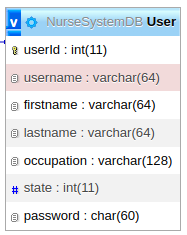
\includegraphics[scale=.6]{./Figures/dB(user).png}
	\caption{Tabla Usuarios.}
	\label{fig:Tabla Usuarios (base de datos)}
\end{figure}

\item Tabla Camas(\textit{Bed}): tabla que contiene la información de las camas como ser su identificación (como en el item anterior se incrementa automáticamente y es clave primaria), ubicación(piso y cuarto) y el número de dispositivo llamador. 

\begin{figure}[ht]
	\centering
	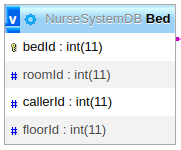
\includegraphics[scale=.6]{./Figures/dB(bed).png}
	\caption{Tabla Camas.}
	\label{fig:Tabla Camas (base de datos)}
\end{figure}

\item Tabla Paciente (\textit{Patient}): tabla que contiene la información de los pacientes. En esta tabla el id no se incrementa automáticamente (ya que puede ser asignado manualmente por el administrador). Ademas, los campos \textit{bedId}, \textit{notesTableId} y \textit{userTableId} contienen claves foraneas que identifican un elemento de la tabla \textit{Bed} (cama), \textit{notesTable} (tablas de notas) y \textit{userTable} (tablas de médicos relacionados al paciente).


\begin{figure}[ht]
	\centering
	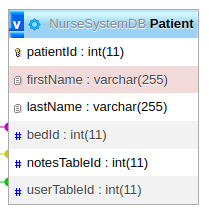
\includegraphics[scale=.6]{./Figures/dB(patient).png}
	\caption{Tabla pacientes.}
	\label{fig:Tabla pacientes (base de datos)}
\end{figure}


\item Relación médicos-pacientes : para generar la relación se utilizan un par de tablas intermedias que permiten que un mismo paciente posea varios médicos tratándolo. Además, un paciente puede utilizar a los mísmos médicos de otro paciente... es una de las ventajas de las bases de datos relacionales.


\begin{figure}[ht]
	\centering
	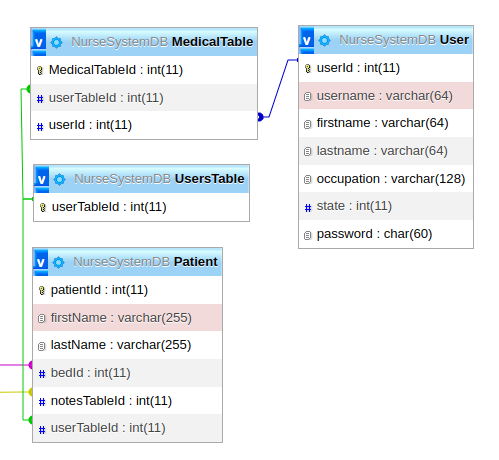
\includegraphics[scale=.40]{./Figures/tabla-medicos-pacientes.png}
	\caption{Relación médicos-pacientes.}
	\label{fig:Relación médicos-pacientes}
\end{figure}



\item Relación tabla de notas- pacientes: como en el caso anterior, se utiliza una tabla de notas generales con una tabla intermedia que los indexa. En este caso y como es particular de cada paciente no se puede repetir.


\begin{figure}[ht]
	\centering
	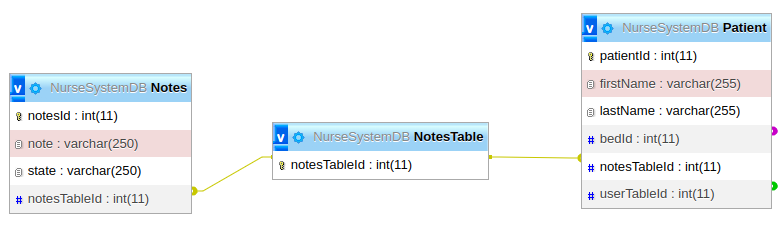
\includegraphics[scale=.45]{./Figures/patient-notes.png}
	\caption{Relación notas-pacientes.}
	\label{fig:Relación notas-pacientes (base de datos)}
\end{figure}

\pagebreak

\item Tabla de eventos programados: En esta tabla se cargan las tareas programadas para un paciente. El identificador se incrementa al generarse, el nro de paciente es enviado por el cliente, el campo tipo de evento puede ser \textit{diario},\textit{mensual} o \textit{anual} y el campo datetime a la hora que se requiere que se realice. El campo nota es donde se coloca la tarea a realizar (Por ejemplo, suministrar X gramos de medicamento Y).


\begin{figure}[ht]
	\centering
	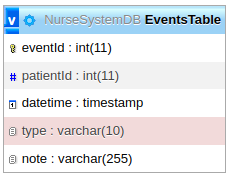
\includegraphics[scale=.45]{./Figures/Events.png}
	\caption{Tabla de eventos programados.}
	\label{fig:Tabla de eventos programados (base de datos)}
\end{figure}


\item Tabla de log eventos: En esta tabla se guardan los eventos relacionados con un paciente. El id se asigna al guardarse el evento. El tipo puede ser \textit{tarea programada} o \textit{llamada paciente}. El id del paciente, el id de usuario y la nota se cargan por el usuario que finalizó la accion.


\begin{figure}[ht]
	\centering
	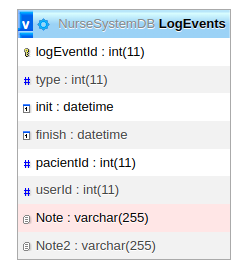
\includegraphics[scale=.45]{./Figures/logEvents.png}
	\caption{Tabla de registro de eventos.}
	\label{fig:Tabla de registro de eventos (base de datos)}
\end{figure}

\item Tabla de especialidades (\textit{SpecTable}): En esta tabla se las distintas especialidades que poseen todos los enfermeros. 

\item Tabla de especialidades de enfermeros (\textit{NurseSpecTable}): En esta tabla se relacionan a los enfermeros con su Id y las distintas especialidades que pueden realizar. Un enfermero puede poseer más de una especialidad.

\item Tabla de tratamientos de pacientes(\textit{PatientSpecTable}): En esta tabla se relacionan a los pacientes con su Id y una tratamiento(se obtiene de la SpecTable). 

\item Tabla de códigos QR (\textit{QRbed}): En esta tabla se almacenan en texto los códigos QR correspondientes a las camas para su reconocimiento.

\item Tabla de prioridades (\textit{PriorityTable}): En esta tabla el administrador puede asignar prioridades a las distintas camas del sistema, las prioridades son de 5 niveles, siendo 5 la más alta prioridad.



\end{enumerate}



\section{Sistema de gestión}

Se diseñó el sistema backend fragmentándolo en tres partes:

\begin{itemize}
\item Monitoreo: clases que ayudan a publicar a todos los clientes MQTT los estados del sistema (usuario logeados y estados de habitaciones/pacientes) 
\item Respuestas al cliente página web: expone una API para que los administradores del sistema puedan incorporar usuarios,pacientes,camas ... observar estadísticas, etc.
\item Respuestas al cliente MQTT: se subscribe a los tópicos correspondientes para responder consultas.
\end{itemize}

En la figura \ref{fig:Estructura de directorio(backend)} se presenta la estructura de directorios del backend.

\begin{figure}[ht]
	\centering
	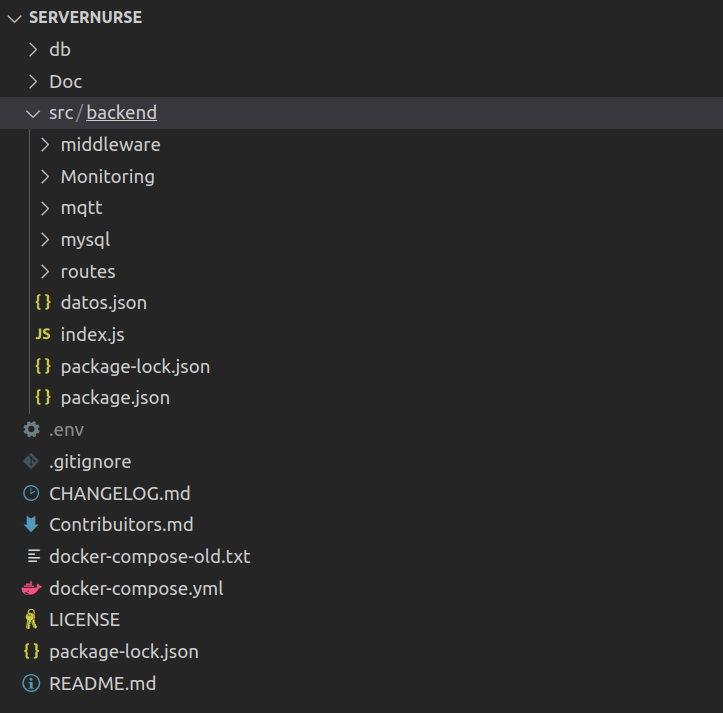
\includegraphics[scale=.45]{./Figures/projectStructure.png}
	\caption{Estructura de directorio (backend).}
	\label{fig:Estructura de directorio(backend)}
\end{figure}

La descripción de los contenidos de cada carpeta es:
\begin{itemize}
\item middleware: contiene el programa que filtra el acceso a la api desde el la página web.
\item Monitoring: contiene clases con información del estado del sistema que se actualiza cada cierto tiempo. Cada una de estas clases contiene una lista de todos los elementos y se presenta a los tópicos correspondientes.
\item mqtt: contiene clases que se encargan de procesar y responder los mensajes que se reciben por medio del protocolo MQTT.
\item mysql: contiene la clase con el \textit{pool} (''grupo'') de conexiones a la base de datos. El objetivo es poder reutilizar conexiones por distintos usuarios.
\item routes: contiene las rutas de express para acceder a la base de datos desde las peticiones por HTTP.
\end{itemize}

\subsection{Descripción de las clases para monitoreo del sistema}

Las siguientes son clases que se utilizan para reportar mediante MQTT los estados del sistema. Para resumir se presentan los elementos principales, pero no las funciones que las componen.

\begin{itemize}

\item \textit{ Monitoreo de camas} \ref{cod:bedlist}:\\
Una  clase llamada \textit{Bedslist} la cual contiente una lista de elementos json con información de cada cama (se instancia al iniciar el backend).

\begin{lstlisting}[label=cod:bedlist,caption=  Clase Bedlist]
class  BedsList  {    
    constructor() {
         this.bedlist=[{id:0,st:0,spec:0}];                        
    }
...}
\end{lstlisting}

Los componentes de cada elemento son 
\begin{enumerate}
\item id: identificador de cama.
\item st: estado de la cama. Puede poseer los siguientes estados: 
\begin{itemize}
\item 0: no ocupada.
\item 1: ocupada.
\item 2: llamando paciente.
\item 3: llamada aceptada por enfermero.
\item 4: enfermero atendiendo.
\item 5: tarea programada.
\item 6: enfermero solicitando ayuda.
\end{itemize}
\item spec: número de tratamiento del paciente en la cama (es utilizado por los clientes enfermeros para filtrar si pueden o no atenderlo).
\end{enumerate}

\pagebreak
\item \textit{ Monitoreo de usuarios:}\\
Una clase \textit{UserList} la cual contiente una lista de elementos json con información de cada usuario (se instancia al iniciar el backend):

\begin{lstlisting}[caption=  Clase Userlist]
constructor() {
         this.UserList=[{id:0,st:0}];                
        
    }
...}
\end{lstlisting}

Los componentes de cada elemento son 
	\begin{enumerate}
		\item id: identificador de usuario.
		\item st: estado de usuario. Puede poseer los siguientes estados: 
			\begin{itemize}
				\item 0: no logeado.
				\item 1: logeado.
			\end{itemize}
	\end{enumerate}




\item \textit{ Monitoreo de eventos programados:}\\
Esta clase se utiliza para presentar a los clientes las notas de tareas programadas que se lanzan. Es una lista que se vacía cuando la tarea finaliza (sirve para mantener ordenadas las tareas programadas).

\begin{lstlisting}[caption=  Clase CalendarList]
constructor() {
         this.CalendarList=[{calendarId:0,bedId:0,note:null}];                
        
    }
...}
\end{lstlisting}

Los componentes de cada elemento son 
	\begin{enumerate}
		\item calendarId: identificador de evento.
		\item bedId: número de cama.
		\item note: Nota de la tarea(obtenida de la base de datos).		

	\end{enumerate}




\item \textit{ Monitoreo de paciente-usuario-tipo de evento:}\\
Esta clase se utiliza para en todo momento saber quien está atendiendo a un paciente.

\begin{lstlisting}[caption=  Clase BedsUserList]
 constructor() {
         this.beduserlist=[{bedId:0,userId:0,type:0}];                        
    }
...}
\end{lstlisting}

Los componentes de cada elemento son 
	\begin{enumerate}
		\item bedId: número de cama.
		\item userId: número de usuario.
		\item type: tipo de evento: 1 llamador, 2 calendario.		

	\end{enumerate}


\end{itemize}
\subsection{Descripción de API MQTT para la mensajería de la aplicación móvil}

El archivo principal es mqtt.js (dentro de la carpeta mqtt) y contiene la inicialización de la conexión inicial al broker, el lanzamiento de las tareas de monitoreo (publicación de las listas antes definidas en los tópicos específicos) y la escucha de los mensajes. Una vez recibido un mensaje, dependiendo del tipo del mismo se deriva los mismo a la clase correspondiente que realiza el tratamiento.



\begin{lstlisting}[caption=  Tareas ejecutadas por mqtt.js]
var client = mqtt.connect(process.env.MQTT_CONNECTION)
//listening to  messages
client.on('connect', function () {
  client.subscribe('/User/#', function (err) {
    if (err) {
    console.log("error:"+err);
    }
  })

  client.subscribe('/Pacient/#', function (err) {
    if (err) {      
      console.log("error:"+err);
    }
  })
  client.subscribe('/Beds/#', function (err) {
    if (err) {      
      console.log("error:"+err);
    }
  })

  //task that will publish beds state each second
  setInterval(publishBedStates, 10000);
  //task that will publish users state 
  setInterval(publishUserStates, 15000);
})
\end{lstlisting}

El sistema recibe mensajería por medio de tres tópicos principales: \textit{User}, \textit{Pacient} y \textit{Beds}. Por otra parte, se utilizan variables de entorno como ser \textit{MQTT\textunderscore CONNECTION}  , que contiene informacion de la IP del broker y el puerto del mismo.

Por último, dentro de esta función se setean dos temporizadores para ejecutar las funciones publishBedStates y publishUserStates que publican los listados de los estados de camas y usuarios cada cierto tiempo.




En general, contenido útil de los mensajes MQTT tiene la siguiente forma:

\begin{lstlisting}[caption=  Formato mensaje MQTT]

payload={_username: "xxxx",_content: "xxx", _bedId: xx, _type: x}

\end{lstlisting}

La descripción de los campos es la siguiente:
\begin{itemize}
\item \textunderscore username: nombre del usuario que envió el comando
\item \textunderscore content: contenido
\item \textunderscore bedId: numero de cama a la que se hace referencia
\item \textunderscore type: tipo de mensaje
\end{itemize}

El tipo de mensaje permite al sistema derivar a las clases correspondientes las tareas a realizar. 

%\begin{verbatim}
\begin{table}[h]
	\centering
	\caption[Tipos de mensajes MQTT]{Tipos de mensajes del sistema.}
	\begin{tabular}{l c c}    
		\toprule
		\textbf{Tipo}     & \textbf{Descripción} \\
		\midrule
		1 & Login.    \\		
		2 & Logout.\\
		3 & Escribir nota a paciente.\\
		4 & Solicitar información de paciente de una cama.\\
		5 & Solicitar notas del paciente. \\
		7 & Mensaje de texto entre usuarios.\\
		8 & Solicitar información de cama (ubicación).\\
		9 & Solicitando información de camas de cada médico.\\
		10 & Solicitar información de un paciente de una cama.\\
		11 & Chequeo de QR.\\
		12 & Aceptación de parte de una enfermera.\\
		13 & Finalización de trabajo.\\
		14 & Solicitar ayuda.\\
		16 & Especialización de enfermera.\\
		17 & Consultar tabla de médicos asignada a paciente.\\
		18 & Eliminar nota de paciente.\\
		19 & Cancelar visita.\\
		20 & Notas de evento calendario.\\
		22 & Mensaje de audio entre usuarios.\\
		\bottomrule
		\hline
	\end{tabular}
	\label{tab:Modelo}
\end{table}
%\end{verbatim}

Las distintas clases que se utilizan son: 
\begin{enumerate}
\item beds: consulta a la base de datos información relacionada a las camas.
\item patient: consulta a la base de datos información relacionada a los pacientes. 
\item users: consulta a la base de datos información relacionada a los usuarios (funciones de logueo y deslogueo).
\item calendar: consulta a la base de datos información relacionada a los eventos programados.
\item nurse: consulta a la base de datos información sobre las especialidades de los enfermeros.
\end{enumerate}

Todas estas clases responden en un tópico correspondiente a los clientes que consultan.


Las excepciones al formato general de los mensajes vienen dadas por:
\begin{itemize}
\item Mensaje de último testamento: informa que un usuario se desconectó. En su \textit{payload} contiene información del nombre de usuario y se publica en el tópico $"/User/Disconnect"$.
\item Mensaje de llamador: informa que un dispositivo llamador fue accionado por un paciente. En su \textit{payload} contiene información del número de llamador y se publica en el tópico $"/Beds/Caller-events"$.

\end{itemize}


\pagebreak

\subsection{Descripción de API REST para aplicación Web}

La API del trabajo utiliza Express junto con Cookie-parser. 
 
En este trabajo se utiliza un \textit{middleware} (capa de software intermedia entre los recursos y la consulta de los usuarios), el cual consiste en una función que realiza el control de acceso a los endpoints. Por definición la página web de configuración solo puede ser accedida por los usuarios administradores, para lograr autenticación el \textit{backend} utiliza las librería \textit{jsonwebtoken} \citep{WEBSITE:32} y \textit{bcrypt} \citep{WEBSITE:31}. 

Se denomina ruteo a la forma que un \textit{endpoint} (punto de acceso, en español) de una aplicación responde a las peticiones de los clientes. En las aplicaciones express, el objeto express posee métodos que realizan las operaciones sobre la base de datos o el sistema.

\begin{lstlisting}[caption=  Rutas express]
app.use('/api/patient',auth.isAuthenticated,routerPatient);
app.use('/api/user',auth.isAuthenticated,routerUser);
app.use('/api/messages',auth.isAuthenticated,routerMessages);
app.use('/api/notes',auth.isAuthenticated,routerNotes);
app.use('/api/beds',auth.isAuthenticated,routerBeds);
app.use('/api/usersTable',auth.isAuthenticated,routerUsersTable);
app.use('/api/medicalTable',auth.isAuthenticated,routerMedicalTable);
app.use('/api/QR',auth.isAuthenticated,routerQR);
app.use('/api/events',auth.isAuthenticated,routerEvents);
app.use('/api/logEvents',auth.isAuthenticated,routerLogEvents);
app.use('/api/Statistics',auth.isAuthenticated,routerStatistics);
app.use('/api/authentication',routerAuthenticate);
app.use('/api/specTable',auth.isAuthenticated,routerSpecTable);
app.use('/api/nurseSpecTable',auth.isAuthenticated,routerNurseSpecTable);
app.use('/api/treatment',auth.isAuthenticated,routerPatientSpecTable);
\end{lstlisting}


La ruta authentication se utiliza para entregar un \textit{token} al cliente, en dicha función se verifica que el usuario sea administrador.

\begin{lstlisting}[caption=  Logueo web]
routerAuthenticate.post('/', async function(req, res) {
    if (req.body) {
        var user = req.body;
        await pool.query('Select username,password,occupation from User WHERE username=?',[user.username], async function(err, result, fields) {
            if (err) {
                var response = JSON.stringify(response_conform);
                res.status(403).send({
                    errorMessage: 'Auth required!'});
                return;    
            }
            else{
                try{
                testUser.username=result[0].username;
                testUser.password=result[0].password;
                }catch (e){res.status(403).send({
                    errorMessage: 'Auth required!'});
                    return;    
                    }
                    await bcrypt.compare(user.password, result[0].password, (err, resultComp)=> {

                        if ((resultComp==true  ) &&(result[0].occupation=="Administrador") ){
                            var token = jwt.sign(user, process.env.JWT_SECRET,{
                                expiresIn: process.env.JWT_EXP_TIM
                            });
                            res.status(200).send({
                                signed_user: result[0],
                                token: token
                            });
                        } else {res.status(403).send({
                                errorMessage: 'Auth required!'
                            }); }
                        })                    
                }      
            }) 
        } else {
            res.status(403).send({
                errorMessage: 'Please provide username and password'
            });
       }

    })


\end{lstlisting}


Luego, la función \textit{auth.isAuthenticated(request,response,next)}, dentro del archivo \textit{./middleware/authentication} filtra el acceso solo a la página web con un usuario administrador logueado.
\begin{lstlisting}[caption=  Control de token]
exports.isAuthenticated = async(req, res,next)=> {
    let authHeader = (req.headers.authorization || '');
    if (authHeader.startsWith("Bearer ")) {
        token = authHeader.substring(7, authHeader.length);
    } else {
        return res.send({ message: 'No Auth' });
    }
    if (token) {
        jwt.verify(token, process.env.JWT_SECRET, function(err) {
            if (err) {
                console.log("Alguien cambio el token, no es valido");
                return res.json({ message: 'Invalid Token' });
            } else {
                console.log("Validado el token y todo ok");
                return next();
            }
        });
    } else {
        return res.send({ message: 'No token' });
    }
}
\end{lstlisting}

Cada recurso posee su ruta correspondiente. Esta forma de organizar el código permite que se incorporen funcionalidades al \textit{backend} de forma sencilla.

\pagebreak

\section{Página Web}

La página web de administración consiste en un \textit{dashboard} (tablero de control) que permite al usuario administrador gestionar el sistema.
Es implementada utilizando el framework Ionic/Angular, con el lenguaje de programación Typescript y las principales áreas de la visualización se observa en la figura \ref{fig:Página web}.

\begin{figure}[ht]
	\centering
	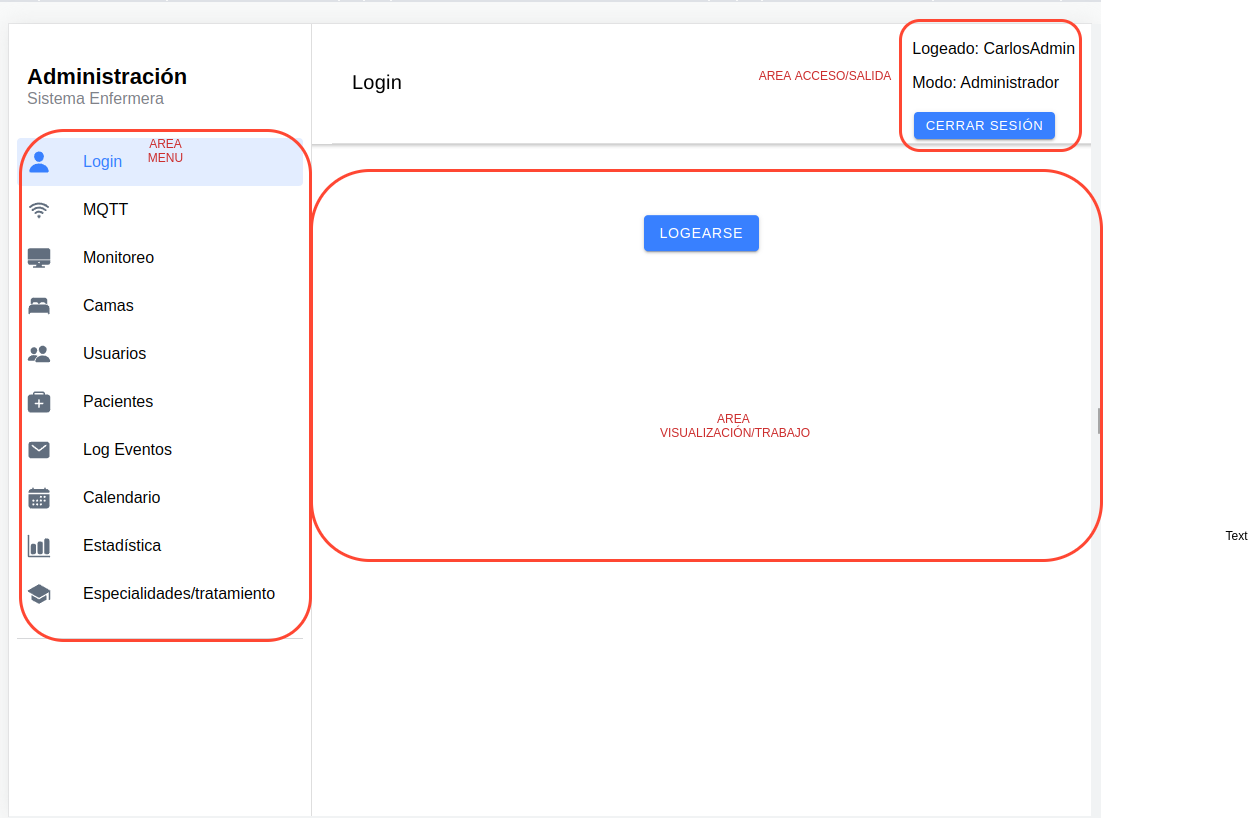
\includegraphics[scale=.48]{./Figures/pagina-web.png}
	\caption{Página web.}
	\label{fig:Página web}
\end{figure}

En el área menú se presentan las distintas utilidades de la página:
\begin{itemize}
\item Login: acceso al sistema. El visitante ingresa su nombre de usuario y contraseña y se le otorga los permisos correspondientes (la conexión recibe el \textit{token} del \textit{backend}).
\item MQTT: permite editar o probar la conexión al broker MQTT del sistema. Es necesario si se desea monitorear el estado de los usuarios o camas en tiempo real.
\item Monitoreo: se visualiza el estado de las camas o de los usuarios en tiempo real.
\item Camas: permite editar información de las camas como ser código QR, numero de llamador, cuarto y piso.
\item Usuarios: permite agregar,editar o dar de baja usuarios.
\item Pacientes: permite agregar,editar o dar de baja pacientes.
\item Log Eventos: permite observar el listado de eventos que se hayan guardado en la base de datos.
\item Calendario: permite observar o agregar tareas rutinarias asignadas a un paciente.
\item Estadísticas: permite observar el numero de intervenciones de un enfermero, la distribucion de especialidades dentro del grupo de enfermeros y la distribución de tratamientos requeridos por los pacientes. Con esta información el administrador puede notificar sobre necesidades de mayor capacitación en un tema para los enfermeros.
\end{itemize}


\subsection{Estructura y organización del software}

El software web generado contiene dos versiones: una para un entorno de desarrollo y otra para un entorno productivo. En este desarrollo, las características del entorno se encuentran en una carpeta \textit{''/src/environments''}. 

Para ejecutar la aplicación en la máquina local se debe ejecutar el comando:  \textit{'' ionic lab ''}, mientras que para compilar la página productiva se debe ejecutar \textit{'' ionic build prod ''}. El resultado de la construcción se encuentra dentro de la carpeta \textit{''/www''}.

Todo el código de la aplicación se encuentra en la carpeta \textit{''/src/app''} y se presenta una captura en la figura \ref{fig:Carpetas página web.}.


\begin{figure}[ht]
	\centering
	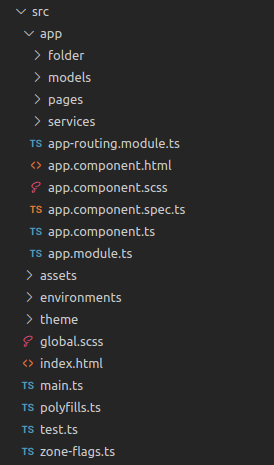
\includegraphics[scale=.60]{./Figures/codigoFront.png}
	\caption{Estructura de carpetas página web.}
	\label{fig:Carpetas página web.}
\end{figure}


Dentro de la carpeta \textit{models} se encuentran las distintas clases que se utilizan para la comunicación con el backend. Las características se presentan a continuación:

\begin{itemize}
\item bed-status: gestiona información del estado de las camas(''ocupada'', ''llamando'',...) y del tratamiento que utiliza el paciente.
\item bed: gestiona información de las camas.
\item calendarEvent: se utiliza para gestionar información de tareas programas.
\item logEvent: se utiliza para gestionar información de eventos realizados.
\item medicalTable: relaciona un usuario con una tabla de médicos.
\item message-model: modelo de mensaje que se transmite a través de MQTT.
\item message: modelo de mensaje almacenado en base de datos(no utilizado).
\item note: modelo de nota para un paciente(no utilizado en la aplicación web).
\item nurseSpec: clase que se utiliza para observar las especialidades de los distintos enfermeros. Propiedades: numero, numero de especialidad y nombre de especialidad.
\item patient: clase que contiene información del paciente (id, nombre, apellido, cama, índice en la tabla de notas, índice en la tabla de médicos)
\item patientTreat: clase que relaciona un paciente con un tratamiento. Propiedades: índice, número de paciente, número de tratamiento y nombre de tratamiento.
\item qr: relaciona un índice con un texto (se utiliza para guardar / recuperar índices de qr)
\item spec: clase que contiene una especialidad/tratamiento. Contiene un índice y un texto con el nombre.
\item user-status: clase que permite obtener desde el sistema el estado de los usuarios (identificación de usuario y estado "logueado"- "no logeado").
\item user: contiene información del usuario (nombre, apellido, ocupación, contraseña, nombre de usuario).
 
\end{itemize}


Dentro de la carpeta \textit{pages} se encuentran las distintas secciones de acción de la página (se presentan en el área de presentación/trabajo).

Dentro de la carpeta \textit{services} se organizan los distintos servicios.

Dentro de la carpeta \textit{folder} se encuentra el layout principal de la página.

La aplicación posee un módulo principal llamado ''app.module''. Utilizando el angular-router, se redirecciona desde cualquier página a una deseada y se presenta dentro del campo de visualización / edición de la pantalla principal. 



\subsection{Acceso de usuario}

Un usuario no puede acceder a las distintas utilidades de la página si no se encuentra logeado o si no es administrador. Todas las consultas al backend necesitan poseer el \textit(token) de autenticación en su encabezado. Esto se logra mediante el servicio interceptor:


\begin{lstlisting}[caption=  Inserción de token]
export class AuthInterceptorService implements HttpInterceptor {

  constructor(private _router:Router) { }

  intercept(req: HttpRequest<any>, next: HttpHandler): Observable<HttpEvent<any>> {
    if (req.url.includes("/authenticate")){
      return next.handle(req);
    }
    const token: string = localStorage.getItem('token');
    let request = req;
	if (token) {
      request = this.addToken(request, token);
      return next.handle(request)
      .pipe(catchError((error: HttpErrorResponse) => {
        let errorMsg = '';
        if (error.error instanceof ErrorEvent) {
          console.log('Client Error');
          errorMsg = `Error: ${error.error.message}`;
        }
        else {
          console.log('Server Error');
          errorMsg = `Error Code: ${error.status},  Message: ${error.message}`;
        }
        console.log(errorMsg);
        return throwError(errorMsg);
      })
      );
    }else{
      return next.handle(request)
      //if i have no token navigate to login
      this._router.navigate(['/login']);
    }    
  }

  private addToken(request: HttpRequest<any>, token: string) {
    return request.clone({
      setHeaders: {
        'Authorization': `Bearer ${token}`
      }
    });
  }
}

\end{lstlisting}

\subsection{Monitoreo del sistema}
Si se quiere monitorear al sistema, es necesario configurar la ubicación del \textit{broker} dentro de la solapa MQTT. El monitoreo de camas se observa en la figura \ref{fig:Monitoreo de camas.}. El sistema reporta el estado de las camas cada un segundo (o cuando hay un cambio abrupto) y el estado de los usuarios cada un segundo y quinientos milisegundos.

\begin{figure}[ht]
	\centering
	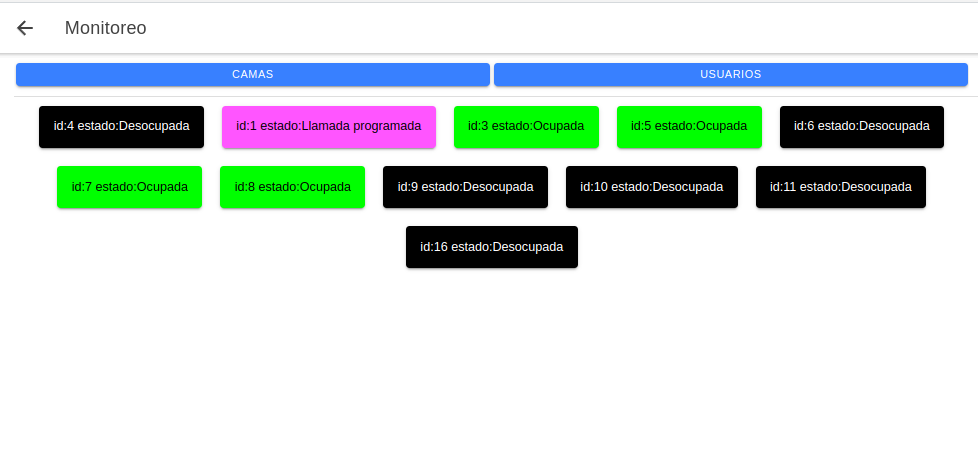
\includegraphics[scale=.40]{./Figures/monitoreo-camas.png}
	\caption{Monitoreo de camas.}
	\label{fig:Monitoreo de camas.}
\end{figure} 

\subsection{Gestión de tareas programadas}

Si se desea generar un nuevo evento programado, se completa el formulario y se presiona enviar.

\begin{figure}[ht]
	\centering
	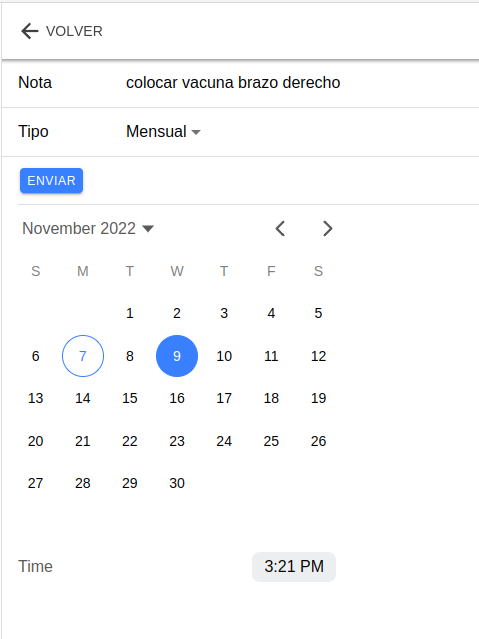
\includegraphics[scale=.40]{./Figures/tarea-programada.png}
	\caption{Tareas programadas.}
	\label{fig:Tareas programadas.}
\end{figure} 

El backend guarda en la base de datos la nueva tarea y genera la acción correspondiente.

\subsection{Estadísticas del sistema}

En esta función se puede observar la cantidad de atenciones por enfermero guardadas en la base de datos, la relación entre las distintas especialidades y la relación entre tratamientos y pacientes. Para generar las graficas se utiliza HighCharts \citep{WEBSITE:33}. 
\begin{figure}[ht]
	\centering
	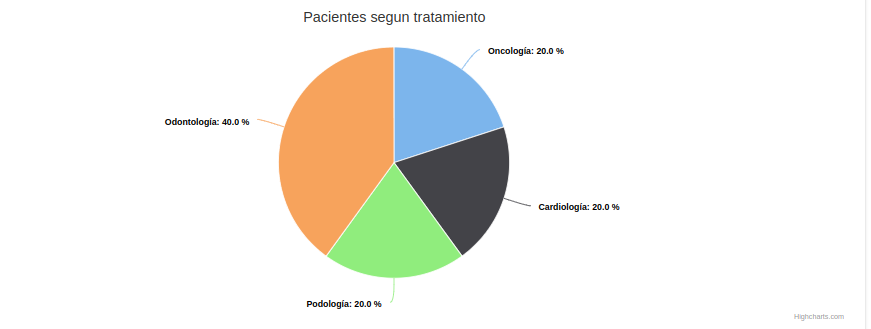
\includegraphics[scale=.40]{./Figures/web/pacientes-Tratamiento.png}
	\caption{Relación paciente tratamiento.}
	\label{fig:Relación paciente tratamiento.}
\end{figure} 


\pagebreak
\section{Aplicación Móvil}
\label{Aplicación Móvil}
En esta sección se presenta la funcionalidad de la aplicación móvil y algunos detalles de la implementación.
\label{Estructura y organización del software}
\subsection{Estructura y organización del software}
La estructura de archivos del proyecto es la presentada en la figura \ref{fig: Estructura de código fuente de la aplicación móvil.}.

\begin{figure}[ht]
	\centering
	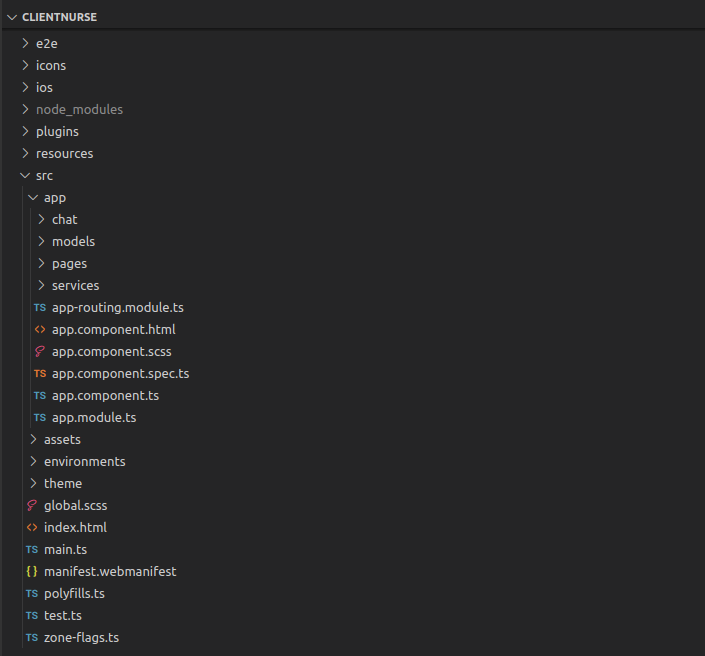
\includegraphics[scale=.60]{./Figures/app/estructura-app.png}
	\caption{ Estructura de código fuente de la aplicación móvil.}
	\label{fig: Estructura de código fuente de la aplicación móvil.}
\end{figure} 

El código de las distintas páginas por las que navega el usuario se encuentra dentro de \textit{''./src/app/pages''}. Los modelos (''clases'') utilizados se encuentra en la carpeta \textit{''./src/app/models''} y los servicios en la carpeta \textit{''./src/app/services''}. La carpeta \textit{''./src/app/chat''} contiene la primera versión la intercomunicación entre enfermeros-médicos que simulaba una sala de reunión (similar a la ofrecida por el producto en el mercado). Luego se migró a la definitiva, que cumple estrictamente con lo solicitado en un principio, pero por solicitud del cliente, no se eliminó la carpeta.

Como se mencionó en secciones anteriores, la aplicación móvil interactua con el backend solo utilizando websockets MQTT.

La aplicación posee un módulo principal llamado ''app.module''. Utilizando el angular-router, se redirecciona desde cualquier página a una deseada. En el código \ref{Rutas de la aplicación móvil}

\begin{lstlisting}[caption=  Fragmento de las rutas de la aplicación móvil]
const routes: Routes = [
  {
    path: 'home',
    loadChildren: () => import('./pages/home/home.module').then( m => m.HomePageModule)
  },
  {
    path: '',
    redirectTo: 'home',
    pathMatch: 'full'
  },
  {
    path: 'mqtt-config',
    loadChildren: () => import('./pages/mqtt-config/mqtt-config.module').then( m => m.MqttConfigPageModule)
  },
  {
    path: 'login',
    loadChildren: () => import('./pages/login/login.module').then( m => m.LoginPageModule)
  },
  ...

\end{lstlisting} 

\pagebreak

\subsection{Configuración del broker y acceso de usuario}

Cuando se inicia la aplicación se presenta una pantalla con dos pulsadores, uno redirige a la página de configuración del broker MQTT y otro a la página de ingreso.
\begin{figure}[ht]
	\centering
	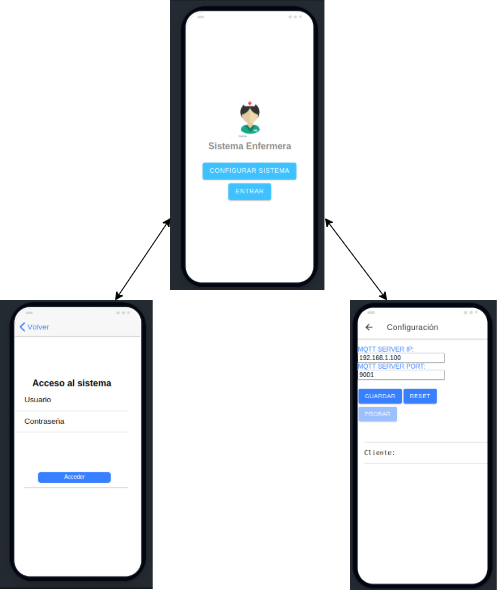
\includegraphics[scale=.80]{./Figures/app/inicioApp.png}
	\caption{ Pantalla inicial, configuración y acceso de la aplicación.}
	\label{fig: Pantalla inicial, configuración y acceso de la aplicación.}
\end{figure} 

En la página de configuración se ingresa la ip del broker del sistema y el puerto. Luego se puede probar la comunicación y guardar los parametros en el localStorage del dispositivo.


\begin{lstlisting}[caption=  Funciones del servicio que guardan en el localStorage]
  /**
   * Saving port values to localStorage
   */
  public saveValues = async () => {     
    this.localSto.saveValuesString('MQTTSERVER',this.MQTTSERVER);
    this.localSto.saveValuesNumber('MQTTPORT',this.MQTTPORT);
  };
\end{lstlisting}

En la página de logueo se ingresan el nombre de usuario, y su contraseña.

La aplicación, publica la información en el tópico ''/User/username'' con el formato de mensaje correspondiente y recibe en ''/Session/nrodesesión'' el número de usuario y el modo de uso. De esta manera la aplicación se configura.


\subsection{Modo administrador}
En el modo administrador se puede monitorear el estado de los usuarios y las camas. Para seleccionar, se presiona el botón correspondiente.

\begin{figure}[ht]
	\centering
	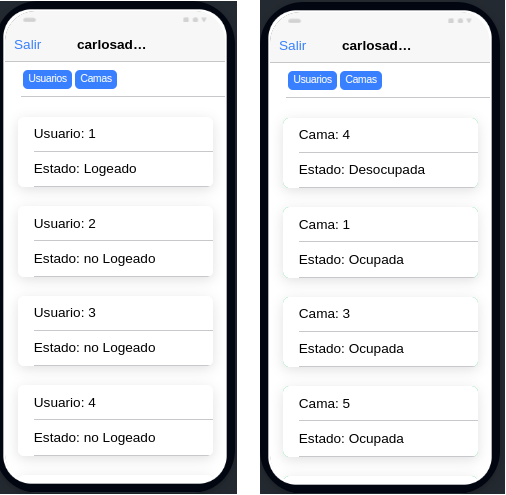
\includegraphics[scale=.70]{./Figures/app/administracion.png}
	\caption{ Pantallas de administración.}
	\label{fig: Pantallas de administración.}
\end{figure} 

El orden en que se presentan las camas tienen que ver con la prioridad que se les asignó a cada una.



\pagebreak
\subsection{Modo médico}
Al ingresar en modo médico, la aplicación queda en modo espera hasta que el usuario decida que hacer. Un diagrama de estados se presenta en la figura \ref{fig: Diagrama de estados en modo médico.}. 

\begin{figure}[ht]
	\centering
	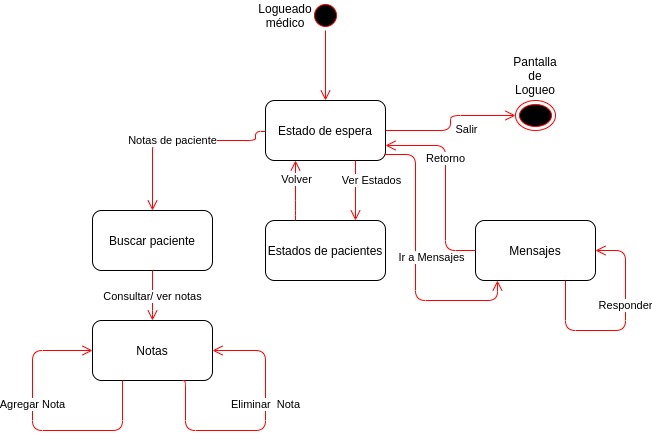
\includegraphics[scale=.60]{./Figures/app/modo-medico.png}
	\caption{ Diagrama de estados en modo médico.}
	\label{fig: Diagrama de estados en modo médico.}
\end{figure} 

Las acciones que puede realizar un médico son:
\begin{itemize}
\item Actualizar una nota de un paciente: para la gestión de estos mensajes se utiliza el tópico ''/Pacient/id'' donde id es el número de paciente. Cuando el médico solicita información del paciente (nombre, apellido y número ) se responde  en ''/Pacient/id/info''. Cuando se consulta las notas se responde en ''/Pacient/id/notes'' y cuando se quiere ingresar una nueva nota se publica en ''/Pacient/id/newNote''
\item Responder a una consulta de una enfermera.
\item Monitorear las camas con los pacientes que le fueron encargados: simplemente filtra por sus pacientes el listado publicado en ''/Beds/status''

\end{itemize}


\begin{figure}[!htpb]
     \centering
     \begin{subfigure}[b]{0.3\textwidth}
         \centering
         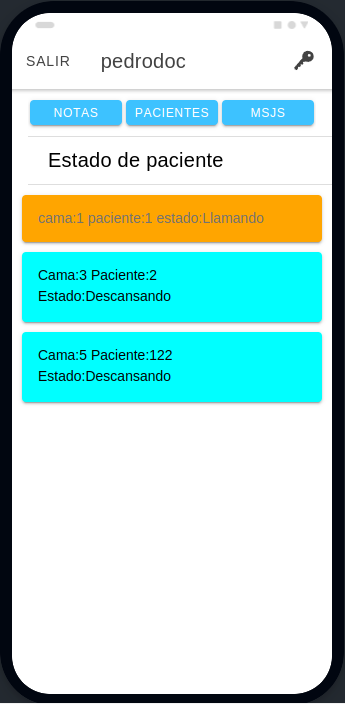
\includegraphics[width=.95\textwidth]{./Figures/app/doctor-patient-1.png}
         \caption{Monitoreo de pacientes.}
         \label{fig_1:1de3}
     \end{subfigure}
     \hfill
     \begin{subfigure}[b]{0.3\textwidth}
         \centering
         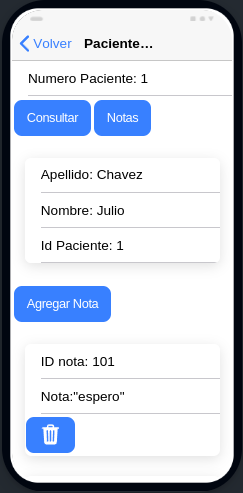
\includegraphics[width=.95\textwidth]{app/doctor-notes5.png}
         \caption{Gestión de notas.}
         \label{fig_1:2de3}
     \end{subfigure}
     \hfill
     \begin{subfigure}[b]{0.3\textwidth}
         \centering
         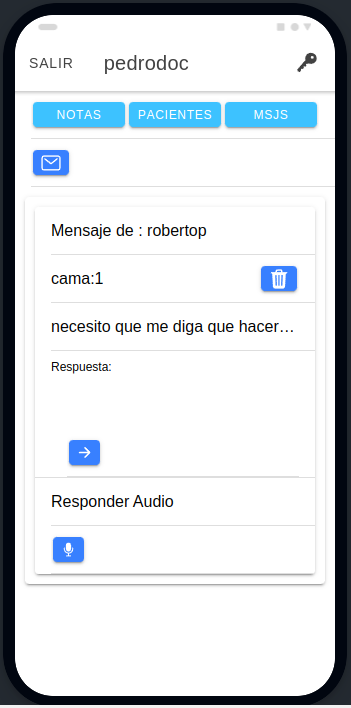
\includegraphics[width=.95\textwidth]{./Figures/app/doctor-message-audio.png}
         \caption{Mensajes.}
         \label{fig_1:3de3}
     \end{subfigure}
        \caption{Modo médico}
        \label{fig:three graphs}
\end{figure}

\pagebreak
\subsection{Modo enfermera}

Es el modo más complejo por la cantidad de opciones que se pueden presentar.

Al ingresar en modo enfermera, se consulta por la especialización del enfermero corresponidente y la respuesta se obtiene de escuchar en el tópico ''/User/userId/Specs''donde userId se recibió al loguearse.

Para el usuario, la aplicación queda en modo espera hasta que se reciba una notificación de necesidad de atención. Un diagrama de estados se presenta en la figura \ref{fig: Diagrama de estados en modo enfermera.}.

 

La aplicación se encuentra escuchando al tópico MQTT ''/Beds/status'', y filtra los estados (solo acepta estados con llamadas , llamadas programadas o ayuda) y por especialidad del enfermero. De esta manera, cuando un enfermero acepta una tarea, automáticamente se actualiza el backend y ningún otro enfermero puede aceptarla.



\begin{figure}[ht]
	\centering
	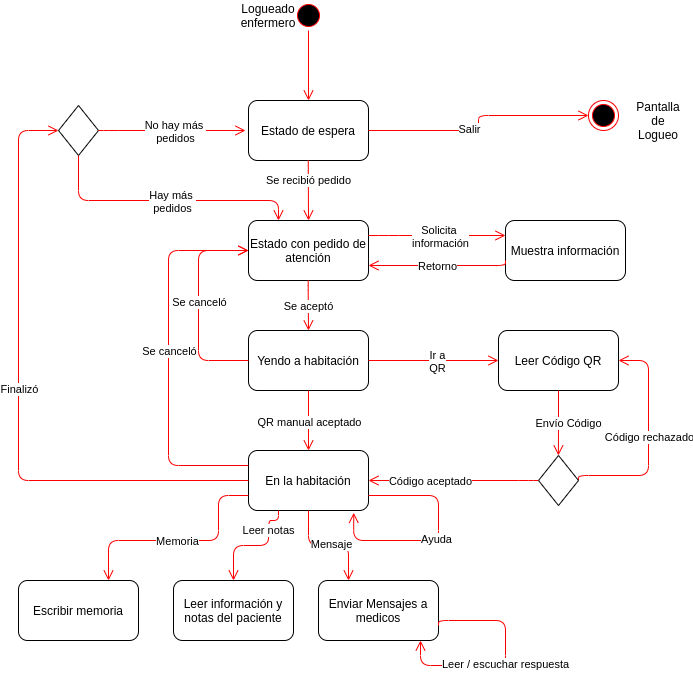
\includegraphics[scale=.60]{./Figures/app/estados-enf.png}
	\caption{ Diagrama de estados en modo enfermera.}
	\label{fig: Diagrama de estados en modo enfermera.}
\end{figure} 


Cuando arriba la notificación, se presenta una tarjeta con dos botones: información de la cama y aceptación. En caso que la enfermera desee consultar donde se encuentra (piso y habitación) debe presionar el boton información. En caso que decida ir a la habitación, debe presionar aceptar.
Al presionar aceptar automáticamente el estado de la cama cambia a desplazandose a la habitación (la información proviene del sistema que recibió la aceptación y cambió el estado de la habitación).


\begin{figure}[!htpb]
     \centering
     \begin{subfigure}[b]{0.3\textwidth}
         \centering
         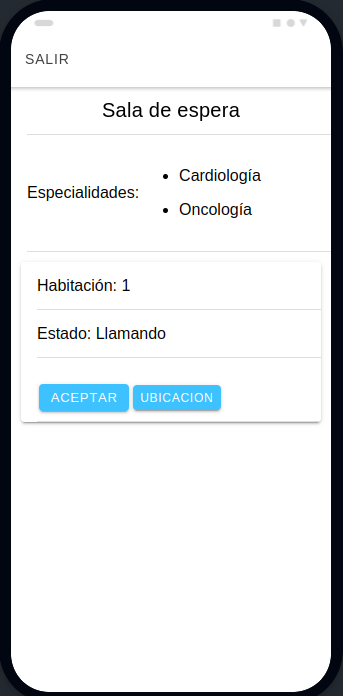
\includegraphics[width=.95\textwidth]{./Figures/app/enfermera-peticion.png}
         \caption{Se recibe peticion.}
         \label{fig_2:1de3}
     \end{subfigure}
     \hfill
     \begin{subfigure}[b]{0.3\textwidth}
         \centering
         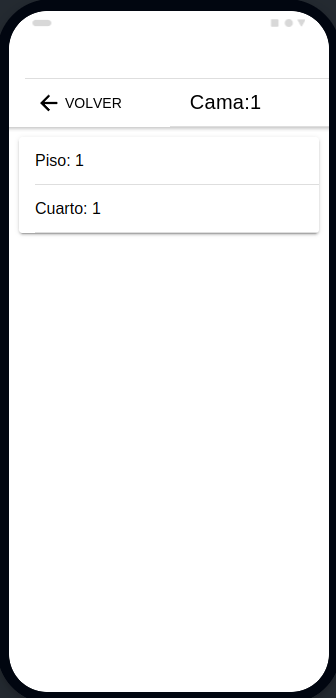
\includegraphics[width=.95\textwidth]{app/enfermera-cama.png}
         \caption{Solicita información.}
         \label{fig_2:2de3}
     \end{subfigure}
     \hfill
     \begin{subfigure}[b]{0.3\textwidth}
         \centering
         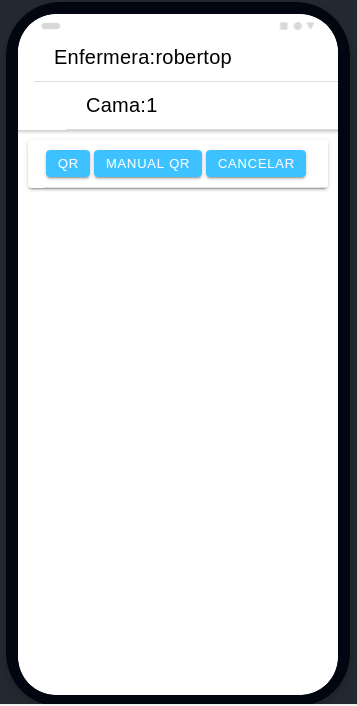
\includegraphics[width=.95\textwidth]{./Figures/app/yendo-enfermera.png}
         \caption{Tarea aceptada.}
         \label{fig_2:3de3}
     \end{subfigure}
        \caption{Recepción de tarea}
        \label{fig_2:three graphs}
\end{figure}
\pagebreak
Cuando el usuario se encuentra frente al paciente, puede ingresar el código correspondiente a la cama manualmente o bien leer el código qr con el celular.



\begin{figure}[ht]
	\centering
	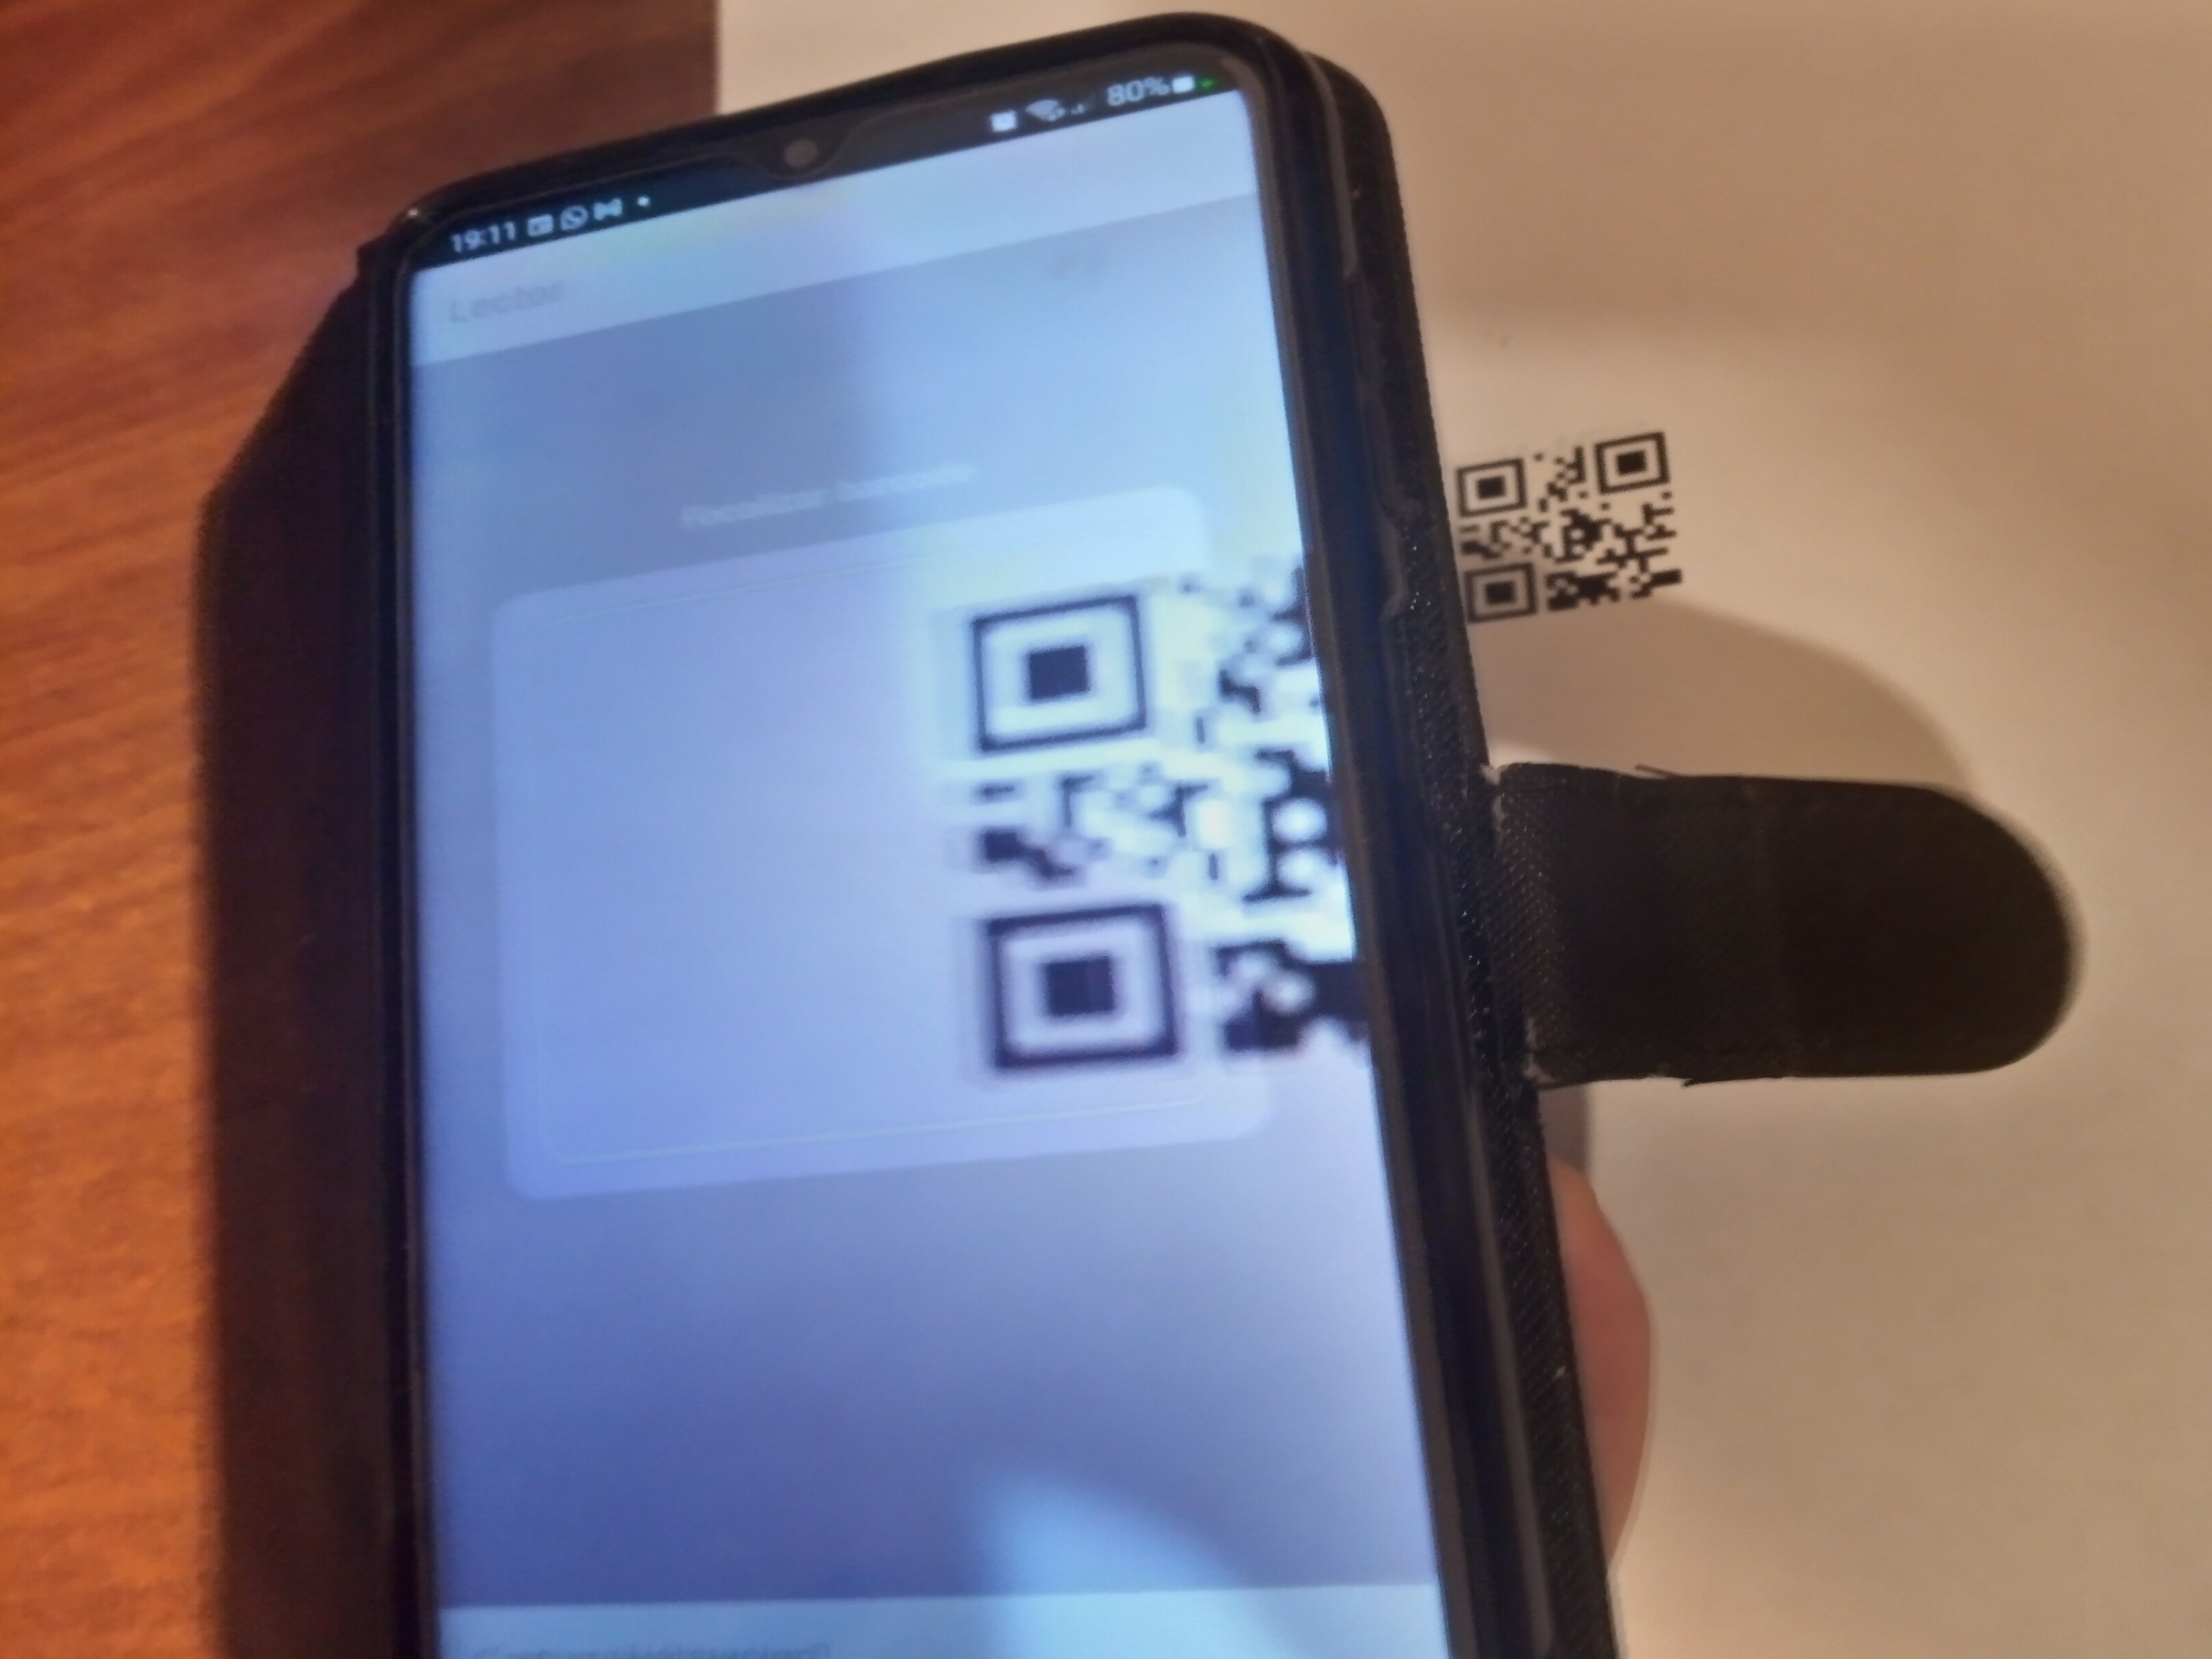
\includegraphics[scale=.10]{./Figures/app/capturaQR.jpg}
	\caption{ Captura de QR en la aplicación}
	\label{fig: Captura de QR en la aplicación.}
\end{figure} 


Una vez que se aceptó desde el sistema el código de la cama, en la aplicación se presenta una pantalla con distintos botones que permiten realizar las siguientes acciones:

\begin{figure}[!htpb]
     \centering
     \begin{subfigure}[b]{0.3\textwidth}
         \centering
         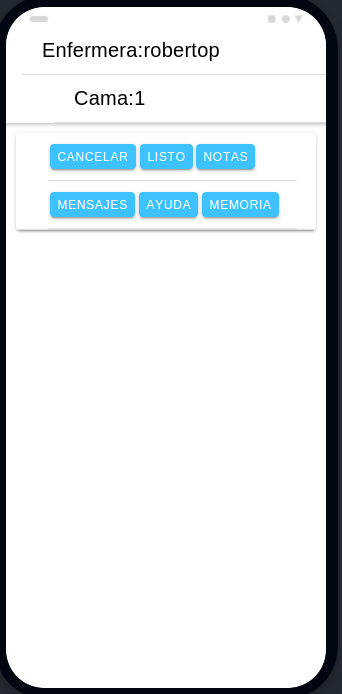
\includegraphics[width=.95\textwidth]{./Figures/app/enfermera-trabajando.png}
         \caption{Menu dentro de habitación.}
         \label{fig_3:1de3}
     \end{subfigure}
     \hfill
     \begin{subfigure}[b]{0.3\textwidth}
         \centering
         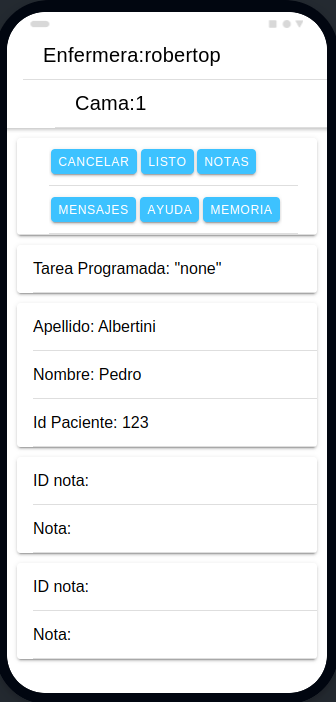
\includegraphics[width=.95\textwidth]{app/enfermera-consultaNotas.png}
         \caption{Solicita información y notas.}
         \label{fig_3:2de3}
     \end{subfigure}
     \hfill
     \begin{subfigure}[b]{0.3\textwidth}
         \centering
         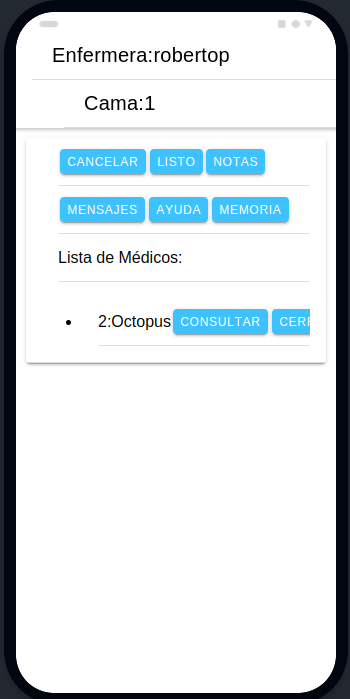
\includegraphics[width=.95\textwidth]{./Figures/app/enfermera-msg.png}
         \caption{Abriendo menú de mensajes.}
         \label{fig_3:3de3}
     \end{subfigure}
        \caption{Ejecución de tarea}
        \label{fig_3:three graphs}
\end{figure}

\begin{enumerate}
\item Cancelar: envía al sistema automáticamente la solicitud de cancelar la tarea. El sistema vuelve a colocar a la cama en situación de llamada.
\item Listo: envía al sistema automáticamente la solicitud de finalizar la tarea. El sistema coloca a la cama en situación de ocupada.
\item Notas: consulta al sistema las notas referidas al paciente. 
\item Mensajes: permite enviar audio o texto a un médico. 
\item Ayuda: solicita al sistema que marque a la cama como con solicitud de ayuda para que otros enfermeros puedan socorrer al usuario. 
\item Memoria: Permite incorporar un texto que se almacena junto con la tarea al presionar Listo.
\end{enumerate}




\pagebreak
\subsection{Interacción médico-enfermera}

\pagebreak
\section{Contraste con los requerimientos}

\subsection{Cumplimiento de requerimientos}

En esta subsección se detalla el grado de cumplimiento de los requerimientos relevados en el plan de proyecto.
\begin{enumerate}
\item Requerimientos del servidor: 

1.1 debe tener instalado el broker mosquitto.

Verificación: Se muesta el funcionamiento del servidor utilizando la aplicación MQTT explorer.

\item Requerimientos de la base de datos: 

2.1 Debe poseer una base de datos relacional. 

2.2 Debe poseer las siguientes tablas: eventos, pacientes, médicos, enfermeras. 

2.2 La base de datos debe poseer datos cargados por default.

Verificación: Se muesta el contendio de la base de datos con la aplicación phpMyAdmin.

\item Requerimientos de la página web 

3.1 Debe ser cliente del broker MQTT. 

Verificación: Se presenta la configuración del broker. Se presenta el monitoreo de las habitaciones y los usuarios conectandose al broker.

3.2 La página debe poseer funciones de consulta o modificación de la base de datos.

Verificación: Se muestra como la página web permite cambiar contraseñas de usuarios y otros parámetros.

3.3 La página debe permitir observar estadística de pacientes y enfermeras.

Verificación: Se muestra como la página web permite observar distintas gráficas.

3.4 La página debe contener acceso con usuario y contraseña para cada persona.


Verificación: Se muestra como la página web permite loguear los distintos usuarios.
(*) Cumplimiento parcial: solo permite loguear al usuario administrador.

\item Requerimientos de la aplicación móvil

4.1 y 4.2 La aplicación debe poseer tres modos de uso: médico, enfermera y sistema. 

Verificación: Se ingresa a la aplicación en los distintos modos.

4.3 La aplicación en modo enfermera debe permitir leer código QR.

Verificación: Se ingresa a la aplicación en modo enfermera y siguiendo los pasos se obtiene el código QR.

4.4 La aplicación en modo enfermera debe descargar información relevante del paciente.

Verificación: Se ingresa a la aplicación en modo enfermera y siguiendo los pasos se descarga las notas del paciente.

4.5 La aplicación en modo sistema debe mostrar las habitaciones sin atención, según una tabla de prioridades y en caso de igualdad de prioridades mostrar según un orden de llamada.

(*)Cumplimiento parcial: se muestra las habitaciones con una tabla de prioridades pero no según el orden de llamadas.

Verificación: Se ingresa a la aplicación en modo enfermera y siguiendo los pasos se descarga las notas del paciente.


4.6 El modo de usuario médico y el modo usuario enfermera deben poder enviar mensajes de texto o sonido.

Verificación: Se transmiten distintos audios entre participantes.

\item Requerimientos de la documentación

5.1 Documento con información relativa a la base de datos: detalles de la misma y API para acceder.

Verificación: Se observa la presencia de la información en el repositorio de GitHub.

5.2 Memoria del proyecto con diagramas de aplicación móvil y página web.

Verificación: se verifica con este documento.

\item Requerimientos de la integración del sistema

6.1 El sistema debe integrar el funcionamiento del servidor con la base de datos, aplicación web y aplicaciones móviles.

Verificación: se verifico el funcionamiento en un laboratorio con 4 usuarios y un simulador de 8 llamadores durante una semana.

(*)Cumplimiento parcial:
Validación: No se pudo validar el sistema en un nosocomio.

\item Requerimientos de la entrega del producto:

7.1 El Código fuente del servidor debe ser subido a dockerhub y compartido con la comunidad.

(*)Cumplimiento parcial:
Validación: Se subió el código fuente del servidor a Github.

7.2 El Código fuente de la aplicación debe ser subido a GitHub y compartido con la comunidad.

Validación: Se subió el código fuente del servidor a Github.

\end{enumerate}
